\apendice{Documentación de usuario}

\section{Introducción}

Esta sección tiene como objetivo proporcionar a los usuarios finales una guía clara y concisa sobre el uso de la aplicación \textbf{VACA} (Voice Assisted Computer Accessibility). Se detallan los requisitos necesarios, el proceso de instalación, y un manual de uso básico para facilitar su adopción.

\section{Requisitos de usuarios}

\subsection{Requisitos del sistema}

Para garantizar el correcto funcionamiento de la aplicación \textbf{VACA}, es necesario cumplir con los siguientes requisitos mínimos, diferenciados entre componentes de software y hardware.

\subsubsection{Requisitos de software}

\begin{itemize}
    \item \textbf{Sistema operativo:} Microsoft Windows 10 o superior.
    \item \textbf{Versión de Python:} Python 3.12 instalado correctamente en el sistema.
    \item \textbf{Dependencias:} Todas las bibliotecas necesarias especificadas en el archivo \texttt{pyproject.toml}, las cuales deben instalarse mediante un gestor compatible como \textbf{Poetry}.
\end{itemize}

\subsubsection{Requisitos de hardware}

\begin{itemize}
    \item \textbf{Micrófono:} Necesario para utilizar las funcionalidades de reconocimiento de voz (STT).
    \item \textbf{Altavoces o salida de audio:} Requeridos para escuchar las respuestas generadas por el sistema mediante síntesis de voz (TTS).
    \item \textbf{Pantallas:} Se recomienda disponer de una configuración de doble monitor. Idealmente, la pantalla principal debe estar situada en el centro y la secundaria a la derecha. Aunque no es estrictamente obligatorio, esta disposición facilita la interacción con el sistema, permitiendo que el usuario visualice el funcionamiento de \textbf{VACA} en la pantalla secundaria, mientras el programa opera sobre la principal.
\end{itemize}

\section{Instalación}
El procedimiento de instalación está pensado para usuarios con conocimientos básicos de informática. Los pasos a seguir son:

\begin{enumerate}
    \item Descargar la última versión de la aplicación desde el repositorio oficial en GitHub: \url{https://github.com/VictorManuelMG/TFGGII_VACA}. \cite{VACARepo}
    \item Instalar \textbf{Python 3.12} desde \url{https://www.python.org/downloads/release/python-3120/}.\cite{python312}
    \item Instalar \textbf{Poetry} como gestor de entornos virtuales, siguiendo la documentación oficial: \url{https://python-poetry.org/docs/}.\cite{poetryDocs}
    \item Definir en \texttt{.env.example} las APIs necesarias.
    \item Abrir una terminal en la carpeta del proyecto y ejecutar el comando \texttt{poetry install} para instalar las dependencias.
    \item Iniciar la aplicación ejecutando el archivo \texttt{gui.py} con el comando \texttt{poetry run python gui.py}.
\end{enumerate}

\section{Manual del usuario}

El uso de la aplicación \textbf{VACA} ha sido diseñado para ser intuitivo. Todas las operaciones se realizan desde la interfaz gráfica integrada que se muestra a continuación:

\begin{figure}[h!]
\centering
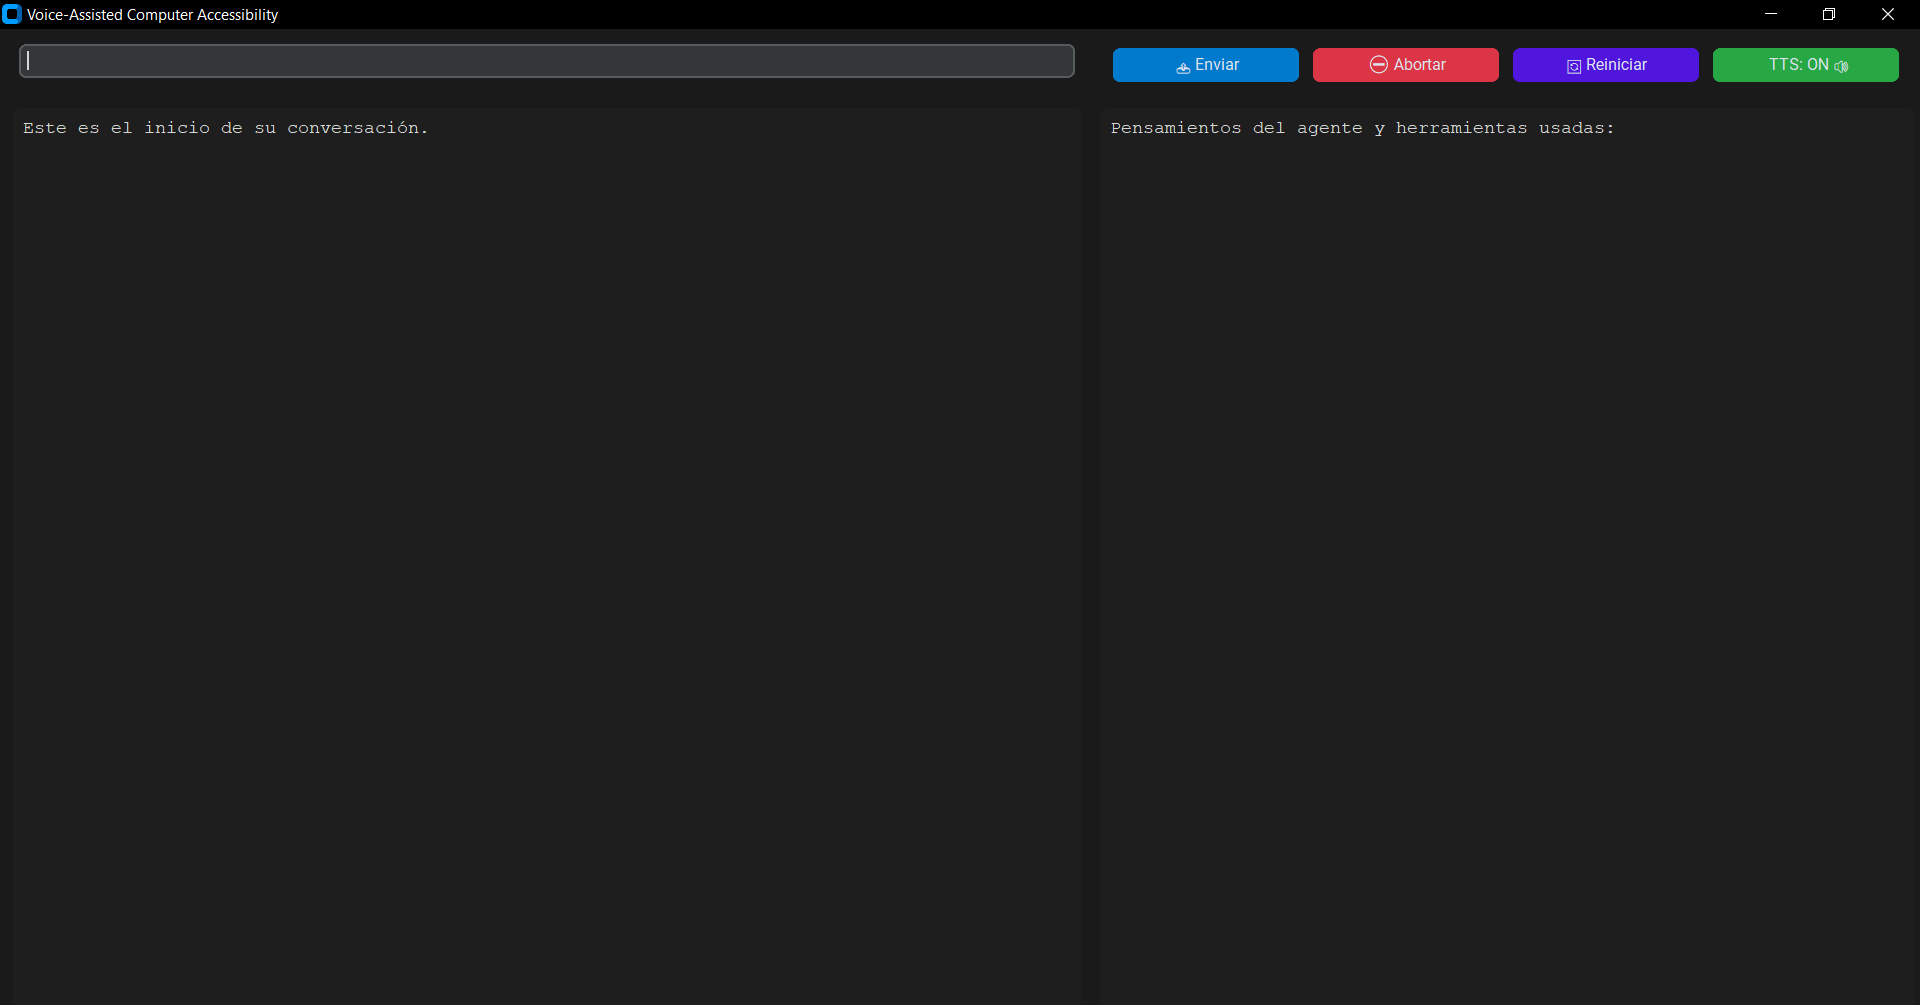
\includegraphics[scale=0.35]{img/interfaz.png}
\caption{Interfaz de usuario.}
\label{fig:manual_interfaz}
\end{figure}

Como puede observarse, la interfaz cuenta con un cuadro de entrada de texto y varios botones con distintas acciones situados en los laterales. El sistema admite entrada de comandos tanto por texto como por voz.

\subsection{Entrada por voz}

\begin{figure}[h!]
\centering
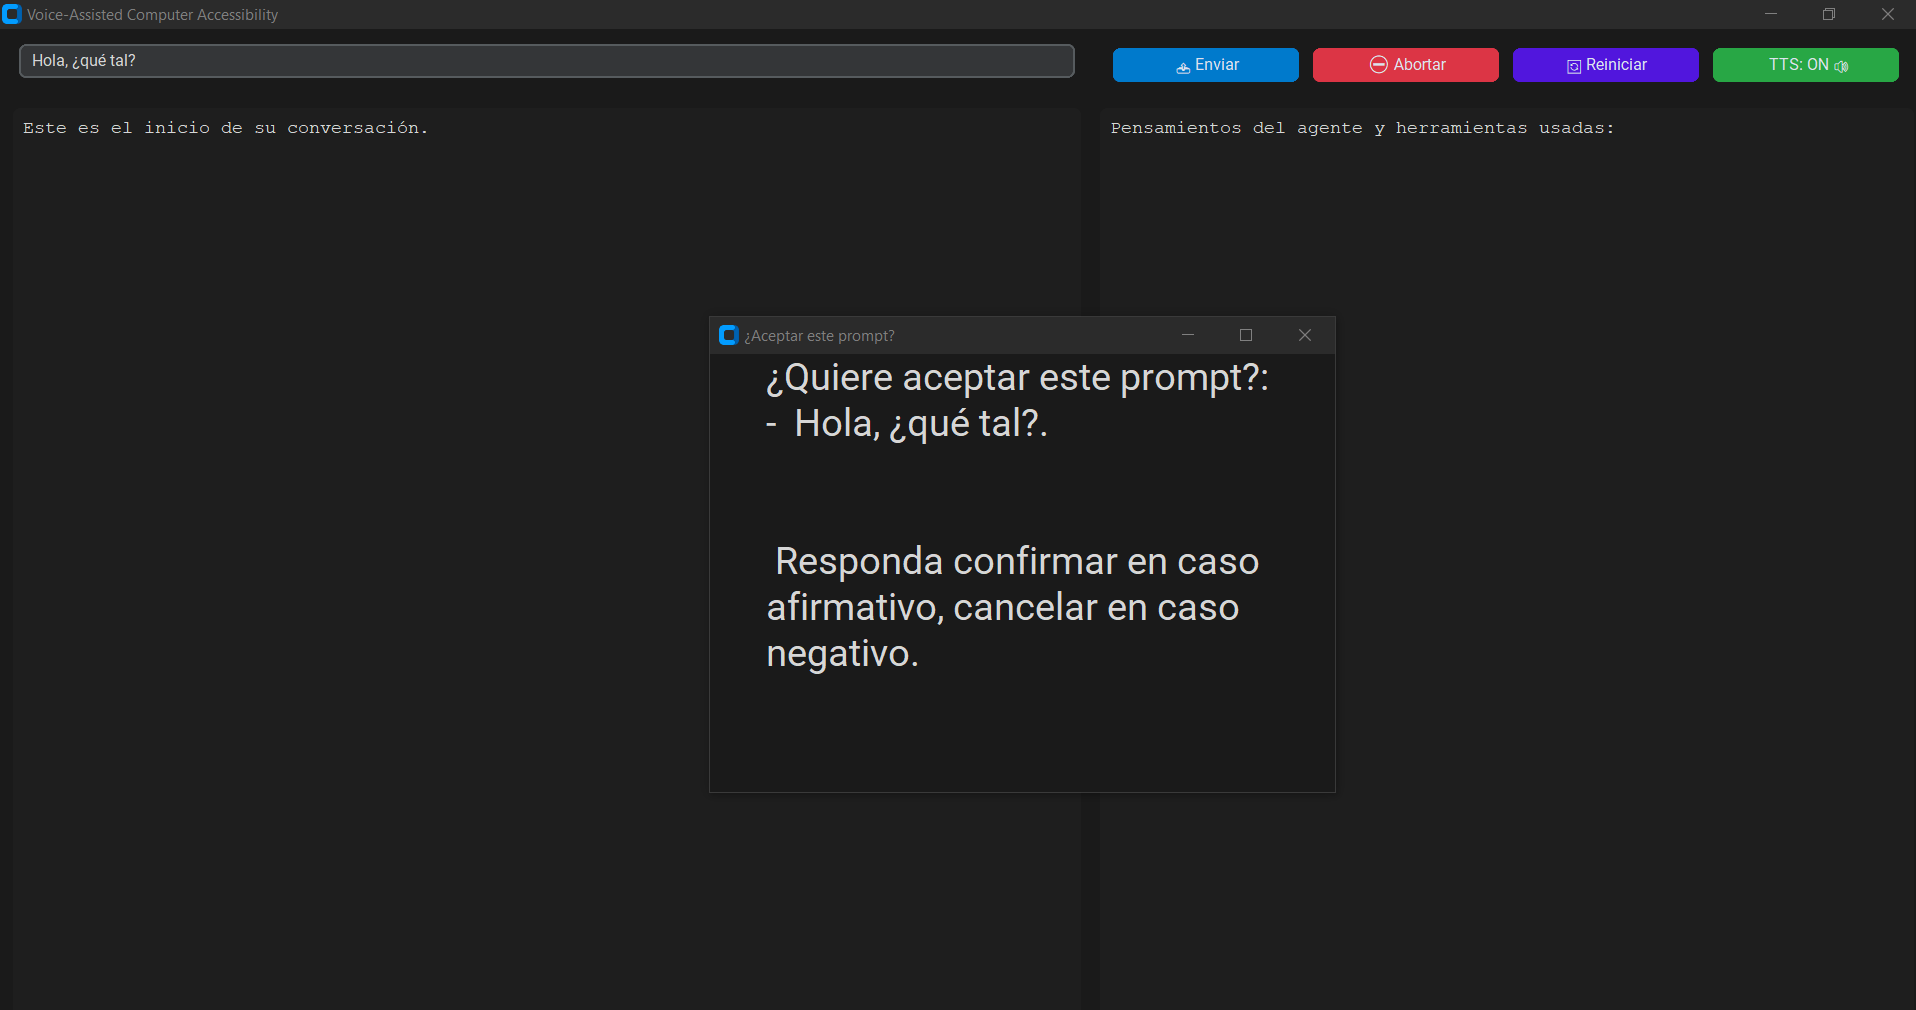
\includegraphics[scale=0.35]{img/input_voz.png}
\caption{Entrada de un prompt mediante voz.}
\label{fig:input_voz}
\end{figure}

Para utilizar esta funcionalidad, basta con hablar al micrófono tras iniciar el programa. Una vez que el comando de voz ha sido capturado y confirmado, el sistema procede automáticamente a procesar la petición del usuario.

\begin{figure}[h!]
\centering
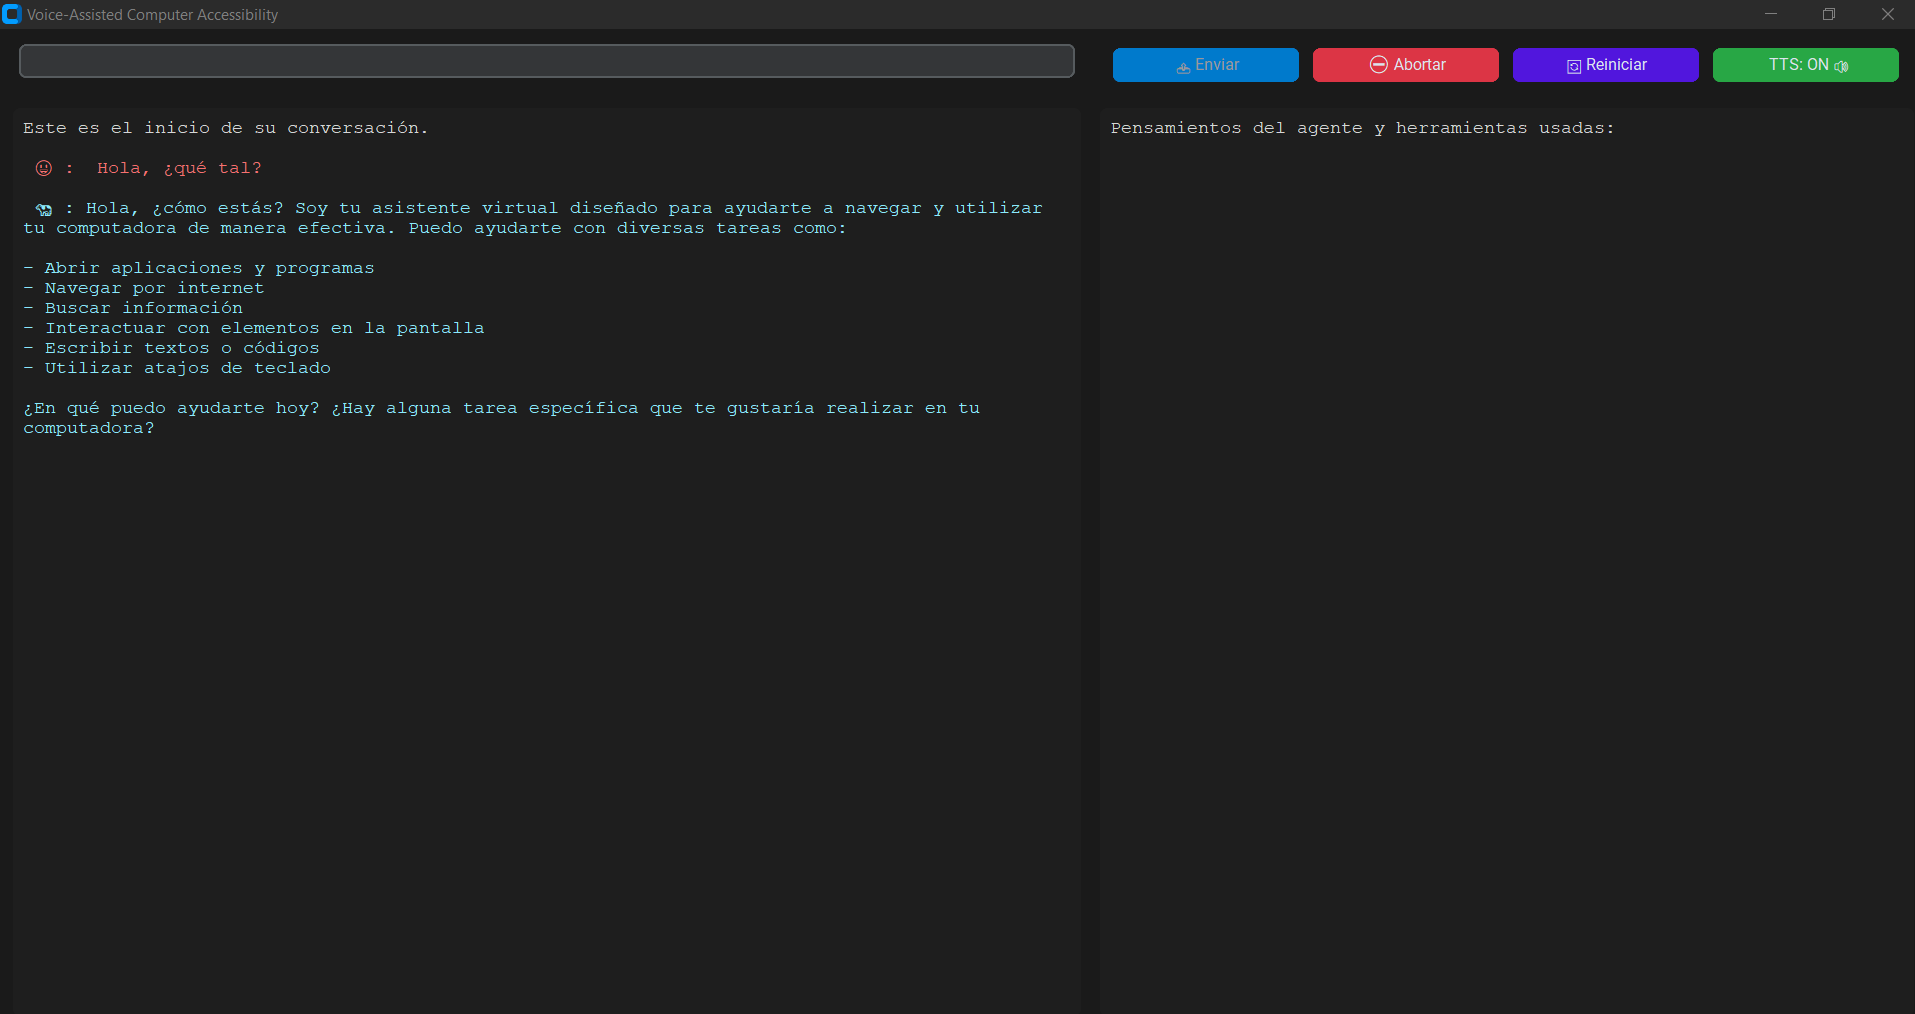
\includegraphics[scale=0.35]{img/Output_voz.png}
\caption{Respuesta generada tras la entrada por voz.}
\label{fig:output_voz}
\end{figure}

Como se muestra en la imagen anterior, tras procesar el prompt, el sistema devuelve una respuesta visual (y opcionalmente también por voz, si el TTS está activado).

\subsection{Visualización de pensamientos del agente}

Además de los resultados visibles de cada acción, el sistema muestra en tiempo real los \textbf{pensamientos del agente}, es decir, los razonamientos internos que realiza al ejecutar determinadas tareas, como la búsqueda de información o el análisis del entorno.

\begin{figure}[h!]
\centering
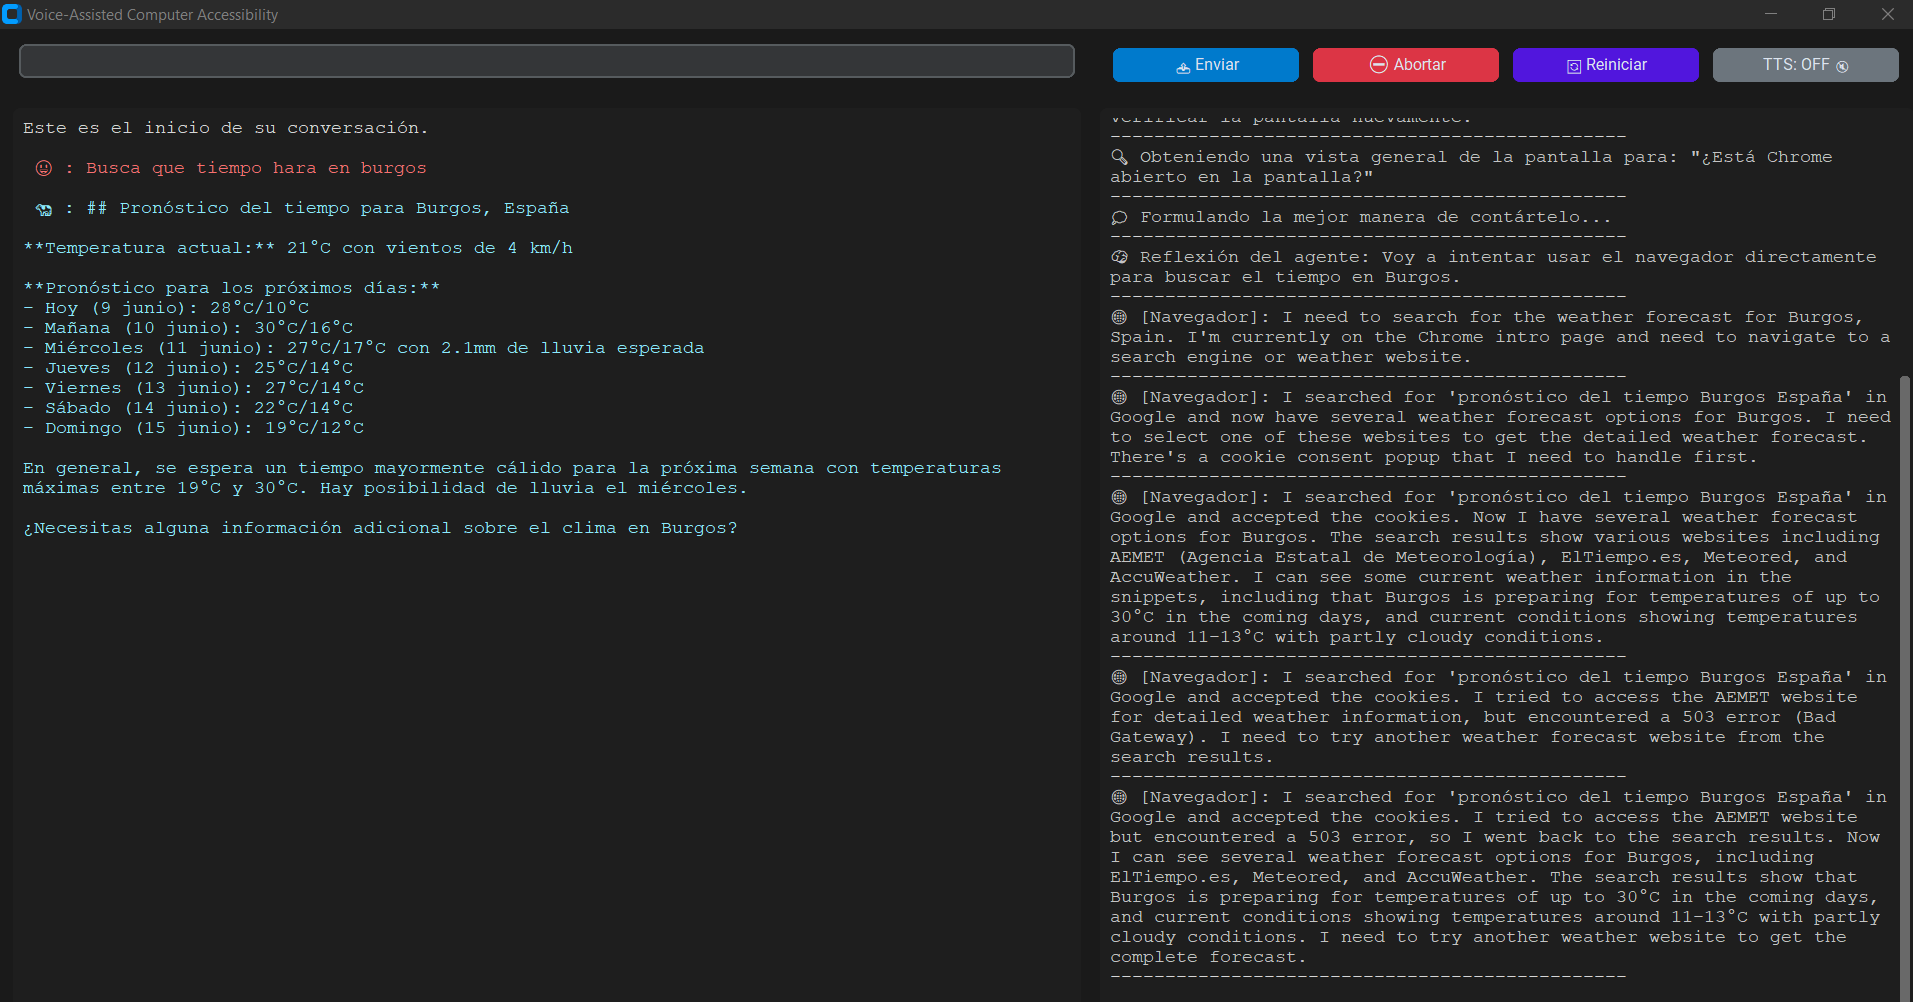
\includegraphics[scale=0.35]{img/Output_search.png}
\caption{Ejemplo de razonamiento mostrado durante una búsqueda en internet.}
\label{fig:output_search}
\end{figure}

Esta funcionalidad permite al usuario comprender mejor qué está haciendo el sistema en cada momento y seguir su lógica de actuación.

\subsection{Recomendaciones de uso}

Se recomienda encarecidamente utilizar un micrófono de buena calidad para garantizar una correcta detección de voz. En caso contrario, podrían producirse errores de reconocimiento. Actualmente, la interfaz no incluye opciones de configuración avanzada del audio, por lo que ajustes como la sensibilidad del micrófono, la ganancia o la amplificación deberán realizarse directamente desde la configuración del sistema operativo.

En futuras versiones se contempla incluir un apartado de configuración accesible desde la propia interfaz para facilitar esta tarea al usuario.